\documentclass[conference]{IEEEtran}
\IEEEoverridecommandlockouts
\usepackage{cite}
\usepackage{amsmath,amssymb,amsfonts}
\usepackage{graphicx}
\usepackage{booktabs}
\usepackage{textcomp}
\usepackage{xcolor}
% Figures and tables are generated by experiments/*.py into results/; keep the repo layout in Overleaf
% (report/ieee/ next to results/) or copy results/figures/*.pdf and results/tables/ieee_*.tex here.
\graphicspath{{../../results/figures/}}
\newcommand{\tab}[1]{\input{../../results/tables/ieee_#1}}

\begin{document}

\title{ParkSight: Forecasting Parking Violations from Enforcement Data That Is Censored by Where Officers Were}

% TODO: confirm full names, department and university before submission.
\author{\IEEEauthorblockN{1\textsuperscript{st} Shaurya Raj Mallick}
\IEEEauthorblockA{\textit{Department, University}\\ City, Country}
\and
\IEEEauthorblockN{2\textsuperscript{nd} Afzal Raja}
\IEEEauthorblockA{\textit{Department, University}\\ City, Country}
\and
\IEEEauthorblockN{3\textsuperscript{rd} Khushi Shorey}
\IEEEauthorblockA{\textit{Department, University}\\ City, Country}
\and
\IEEEauthorblockN{4\textsuperscript{th} Abdul Azeem}
\IEEEauthorblockA{\textit{Department, University}\\ City, Country}
}

\maketitle

\begin{abstract}
A parking ticket exists only where an officer was. In 298{,}445 Bengaluru tickets (54 police stations, 151 days) the number of active enforcement devices falls from 1{,}773 at 11:00 to 12 at 19:00, so ticket counts say little about the evening. We use classical machine learning only and ask three questions. (1) Is the evening gap real? (2) On a semi-synthetic benchmark with a known truth, how much does this censoring hurt, and does inverse-propensity weighting recover the truth? (3) Which classical models forecast next-day station counts and next-week hotspots, and are their intervals honest? At real severity naive counts miss 78\% of the tickets; weighting with the true exposure removes the bias but only if the weight cap is large, and an exposure curve estimated from the thinned data stays almost as biased as the naive count (\(-71\%\)). For counts, a lasso on \(\log(1{+}y)\) reaches a macro MASE of 0.697 against 0.967 for ``same weekday last week''; for hotspots, classifiers reach a PR-AUC of about 0.80 against 0.743 for ranking by last week's impact. Per-tier conformal intervals restore the nominal 80\% coverage that a single global interval misses for the busiest stations (61\%).
\end{abstract}

\begin{IEEEkeywords}
parking enforcement, censored data, inverse-propensity weighting, count forecasting, hotspot classification, conformal prediction
\end{IEEEkeywords}

\section{Introduction and Related Work}
Cars parked on main roads and near junctions squeeze the carriageway and slow traffic, yet enforcement is mostly reactive: officers patrol usual routes and write tickets. The tickets are the only large record of the problem, and a ticket records the presence of an officer as much as the presence of an offence. A model trained on counts learns where officers went, and recommending them to go there again is the feedback loop described for predictive policing by Ensign et al.~\cite{ensign2018runaway}. The loop is not only about location: in our data it is also about \emph{time}. Officers almost vanish in the evening rush, so the evening is exactly the period that is least observed.

\textbf{Related work.} Gao et al.~\cite{gao2019parking} forecast the spatio-temporal legality of on-street parking with random forests on open data; we replicate that model family on a different city and add an explicit treatment of censoring. Learning from data that are observed with unequal probability is the subject of inverse-propensity weighting~\cite{horvitz1952generalization}, applied to debiasing learning and evaluation by Schnabel et al.~\cite{schnabel2016recommendations}; the known difficulty is variance when the observation probability is small, which is the regime of the Bengaluru evening. For uncertainty we use split-conformal prediction~\cite{lei2018distribution}. Tree ensembles are often assumed to dominate tabular prediction~\cite{grinsztajn2022tree}; we test this on both tasks against strong baselines.

\textbf{Contributions.} (i) Device-level evidence of the evening gap. (ii) A semi-synthetic censoring benchmark with known truth that tests weighting and its cap. (iii) A time-blocked comparison of classical models on next-day station counts and next-week hexagon hotspots, always reported against the baselines ``same weekday last week'' and ``last week's impact'' with per-station (macro) metrics. (iv) Global and per-tier split-conformal intervals. ParkSight began as a hackathon project by one author (data pipeline, impact score, a LightGBM forecast); the tasks, folds, metrics, model comparison, benchmark and conformal analysis here were written for this course.

\section{Methodology}
Figure~\ref{fig:method} gives the pipeline. Two parts share the same cleaned tickets: a forecasting pipeline (E3 to E5) and a censoring benchmark (E2).

\begin{figure*}[t]
\centering
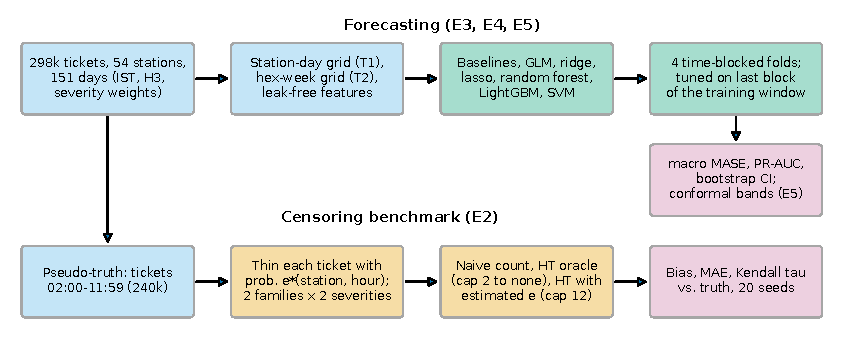
\includegraphics[width=\textwidth]{F0_method}
\caption{Methodology. Top: tickets become two leak-free grids, a model ladder is evaluated on four time-blocked folds with hyperparameters tuned only on the last block of each training window, and results are scored with per-station metrics and conformal bands. Bottom: a well-covered pseudo-truth is thinned with a known exposure curve, then recovered by three estimator families.}
\label{fig:method}
\end{figure*}

\subsection{Data and Prediction Tasks}
Each ticket has a timestamp (converted from UTC to IST), police station, H3 hexagon, a severity weight, a peak-hour weight and an anonymised device identifier. \textbf{T1 (counts):} for each station and day \(d\), predict the count on \(d\) from days before \(d\): counts 1, 7 and 14 days back, 7- and 28-day rolling means, an expanding same-weekday mean, calendar flags and the station. \textbf{T2 (hotspots):} for each H3 resolution-8 hexagon and week \(w\) (21 full weeks), predict whether the hexagon is in the top 10\% of hexagons by weekly impact \(\sum \text{severity}\times\text{peak weight}\) in week \(w{+}1\); features are impact in weeks \(w\) to \(w{-}3\) and their mean, evening share, mean severity, junction share and the mean impact of the six neighbouring hexagons. Every feature uses only earlier data, and a unit test changes all values from a day onward and checks that no earlier feature moves.

\subsection{Models}
\textbf{T1.} Baselines: seasonal naive (the count one week earlier) and a 7-day moving average. Models: Poisson GLM, ridge~\cite{hoerl1970ridge} and lasso~\cite{tibshirani1996lasso} on \(\log(1{+}y)\), a random forest~\cite{breiman2001random} with Poisson splitting, and LightGBM~\cite{ke2017lightgbm} with a Poisson objective. \textbf{T2.} Baselines: persistence (last week's label) and persistence by impact (rank of last week's impact, the stronger one). Models: L2 logistic regression, a calibrated linear SVM, a random forest and LightGBM. Each model has one hyperparameter with 4 to 5 candidate values (penalty, leaf size or number of boosting rounds), chosen on the last 14 days (T1) or 2 weeks (T2) of the training window, never on the test block.

\subsection{Censoring Benchmark}
On real data the unobserved evening has no ground truth, so recovery is tested on a semi-synthetic task. The pseudo-truth is every ticket from 02:00 to 11:59 (240{,}352 tickets), a period with many active devices. Each ticket is kept independently with probability \(e^*(\text{station},\text{hour})\), the shape of the real evening exposure dip mapped onto these hours and scaled so the best hour keeps everything, raised to a \emph{severity} exponent (1.0 is the real severity, 0.5 is milder). The \texttt{same\_for\_all} family uses one curve; \texttt{station\_hetero} gives each station its own random exponent. Estimators: \emph{naive} (count what remains); \emph{HT oracle}, weighting each kept ticket by \(\min(1/e^*,\text{cap})\) with caps 2, 5, 12, 50 and none; and \emph{HT estimated}, which estimates \(e\) from the thinned tickets as distinct devices per hour divided by the maximum (the hackathon method, cap 12). Scores are the relative bias of the total, MAE per station-hour cell, and Kendall's \(\tau\) of the station ranking, over 20 seeds, with bias\(^2\) and variance across seeds reported for the cap sweep.

\subsection{Metrics and Conformal Intervals}
The headline T1 metric is the macro MASE~\cite{hyndman2006another}: per station, absolute error divided by that station's training-window seasonal-naive MAE, then averaged over stations, so one very busy station cannot decide the result (1.0 equals the seasonal-naive forecast). We also report RMSE and mean Poisson deviance, with 95\% bootstrap intervals over stations and paired Wilcoxon tests on per-station MASE. T2 uses PR-AUC (prevalence is 10\%) with a cluster bootstrap over hexagons, F1 at the threshold with the best inner-validation F1, and Brier score, on all hexagons and on the \emph{emerging} subset (not hotspots in week \(w\)). Intervals use split-conformal prediction with quantile level \(\lceil (n{+}1)(1{-}\alpha)\rceil/n\), \(\alpha=0.20\), calibrated on the 21 days before each training end, either with one global quantile or one per station-volume tier (terciles of training ticket totals).

\section{Experimental Settings}
\textbf{Data.} 298{,}445 tickets, 54 stations, 10 Nov 2023 to 8 Apr 2024. The station-day grid has 54\(\times\)151 cells (6.1\% zeros, which are real zeros); the hexagon-week grid has 16{,}275 cells with 10.1\% hotspots.

\textbf{Folds.} Expanding-window, time-blocked, never shuffled. T1 uses four 14-day test blocks starting 13 Feb, 27 Feb, 12 Mar and 26 Mar 2024; T2 uses four 2-week blocks over weeks 13 to 20 of the 21 full weeks. Training rows are strictly earlier than test rows.

\textbf{Seeds and tuning.} Random forest and LightGBM run with seeds 0, 1 and 2; the other models are deterministic. The benchmark uses seeds 0 to 19 and the bootstrap seed is 12345 (2{,}000 resamples over stations; 1{,}000 over hexagons for T2). LightGBM uses the hackathon settings (learning rate 0.04, 24 leaves, subsample 0.85) and tunes only the number of rounds. The grids were widened once after the first version chose the edge of a 3-value grid; chosen values are saved with the results.

\textbf{Reproducibility.} Every number comes from a CSV written by one script per experiment (\texttt{experiments/}); \texttt{run\_all.py} reproduces everything, and device-level data is never committed. Models are classical (scikit-learn and LightGBM); there is no GPU and no neural network, and the full pipeline runs on a laptop CPU.

\section{Results and Ablation Studies}
\subsection{The Evening Gap (E1)}
Tickets fall from 32{,}580 in the 10:00 hour to 27 at 19:00, and active devices from 1{,}773 (11:00) to 12 (19:00); the two curves move together (Figure~\ref{fig:gap}), so the gap is a drop in enforcement presence rather than in violations that we could observe. Two data caveats follow from the device file. Every timestamp has its seconds field equal to 46 (an anonymisation artifact), and 34\% of tickets fall between 00:00 and 06:00 IST; the average device-day runs from about hour 6.6 to hour 8.1 (1.5 hours), so ``evening'' is defined on the recorded clock and we cannot rule out a fixed offset. PCA of the 54\(\times\)24 hourly-share matrix shows that stations differ in \emph{when}, not how much, they record: PC1 explains 30.3\% of variance and K-Means (silhouette 0.21, weak) splits 35 pre-dawn from 19 late-morning stations.

\begin{figure}[t]
\centering
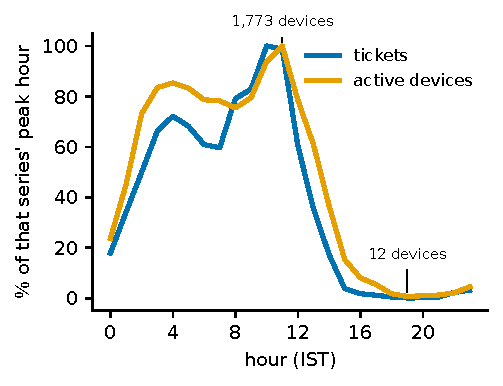
\includegraphics[width=\columnwidth]{F1_evening_gap}
\caption{Tickets and distinct active devices by hour (IST), each indexed to its own peak.}
\label{fig:gap}
\end{figure}

\subsection{Censoring Benchmark (E2)}
Table~\ref{tab:bench} and Figure~\ref{fig:bench} show recovery of the pseudo-truth at real severity. The naive count misses 78\% of the tickets. HT with the true exposure is unbiased only when the cap is large: the hackathon cap of 12 still leaves a \(-42\%\) bias at real severity (but \(\approx 0\) at severity 0.5), cap 50 leaves \(-14.5\%\), and no cap removes the bias (\(+0.1\%\)) at the price of the largest variance: 17{,}817 tickets\(^2\) per cell against 1{,}416 at cap 12, and a station-ranking \(\tau\) that is lower than at cap 50 (0.92 vs 0.93). Capping therefore trades variance for bias, and the cap that looks safe is the one that hides the bias. When \(e\) is estimated from the thinned tickets the result is no better than the naive count (\(-71\%\), \(\tau\) 0.84): at 09:00 the estimate is 0.124 where the true exposure is 0.009, an overestimate of about 14 times, because the estimator uses the same scarce tickets it is meant to correct (the circularity). Station-specific curves lower \(\tau\) for every single-curve method (naive 0.80 to 0.74).

\begin{table}[t]
\centering
\caption{Recovery at severity 1.0: relative bias of the total (\%) / MAE per station-hour cell / Kendall \(\tau\) of the station ranking, mean of 20 seeds.}
\label{tab:bench}
\footnotesize
\tab{bench}
\end{table}

\begin{figure*}[t]
\centering
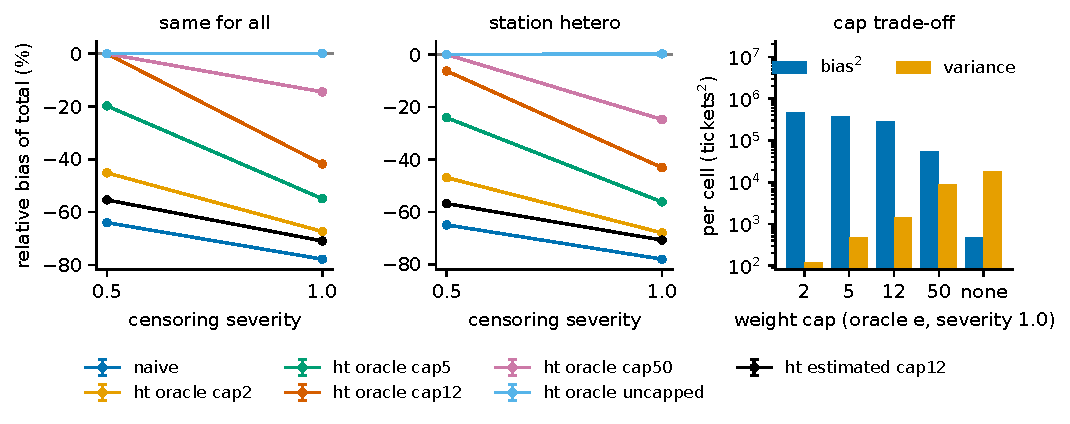
\includegraphics[width=0.95\textwidth]{F2_benchmark}
\caption{Censoring benchmark. Left and middle: relative bias of the total against censoring severity for each estimator (20 seeds; intervals are drawn but narrow). Right: bias\(^2\) and variance across seeds for each weight cap at severity 1.0 (log scale).}
\label{fig:bench}
\end{figure*}

\subsection{Next-Day Counts (E3)}
Table~\ref{tab:counts} compares the T1 models. Every model beats the seasonal-naive baseline (macro MASE 0.967; Wilcoxon \(p<10^{-9}\)). The best are the linear models on \(\log(1{+}y)\): lasso 0.697 [0.642, 0.762] and ridge 0.699, ahead of the random forest (0.730), LightGBM (0.733), the Poisson GLM (0.744) and the moving average (0.750). Lasso and ridge beat the forest station by station (\(p=0.003\), 0.002), LightGBM and the forest are indistinguishable (\(p=0.72\)), but the intervals of the top five models overlap and the 12 tests are uncorrected, so the order within that group should not be over-read. The metrics disagree on the winner: the forest has the lowest RMSE (29.7) and deviance (14.6), which are dominated by the few busiest stations, while MASE weights every station equally; we have not tested this explanation, so macro MASE is the headline. We therefore do not find that tree ensembles dominate here.

\begin{table}[t]
\centering
\caption{T1, next-day counts, four time-blocked folds. Macro MASE (lower is better, 1.0 = seasonal naive) with a 95\% bootstrap interval over stations; RMSE and mean Poisson deviance (Dev.).}
\label{tab:counts}
\footnotesize
\tab{counts}
\end{table}

\subsection{Next-Week Hotspots (E4)}
Hotspots persist, so the question is what a model adds (Table~\ref{tab:hot}, Figure~\ref{fig:pr}). Persistence of the label scores 0.479 PR-AUC; the stronger persistence by impact scores 0.743 [0.664, 0.804]. All four classifiers improve on it, SVM 0.811, logistic regression 0.807, random forest 0.805, LightGBM 0.804, a gain of \(+0.061\) to \(+0.068\) whose bootstrap intervals exclude zero, but the models are indistinguishable from each other and the linear ones match the trees. On the harder emerging subset (208 positives among 5{,}455 rows, 3.8\%) the baseline reaches 0.248 and the classifiers 0.358 to 0.374, a gain of \(+0.110\) to \(+0.126\); absolute F1 stays between 0.24 and 0.31, so new hotspots are ranked better than by the baseline but not found reliably. With four folds, differences below about 0.05 PR-AUC are not evidence.

\begin{table}[t]
\centering
\caption{T2, next-week hotspots (top 10\% by weekly impact). ``Emerging'' keeps hexagons that were not hotspots in the origin week; its F1 for the baselines is 0 by construction.}
\label{tab:hot}
\footnotesize
\tab{hot}
\end{table}

\begin{figure}[t]
\centering
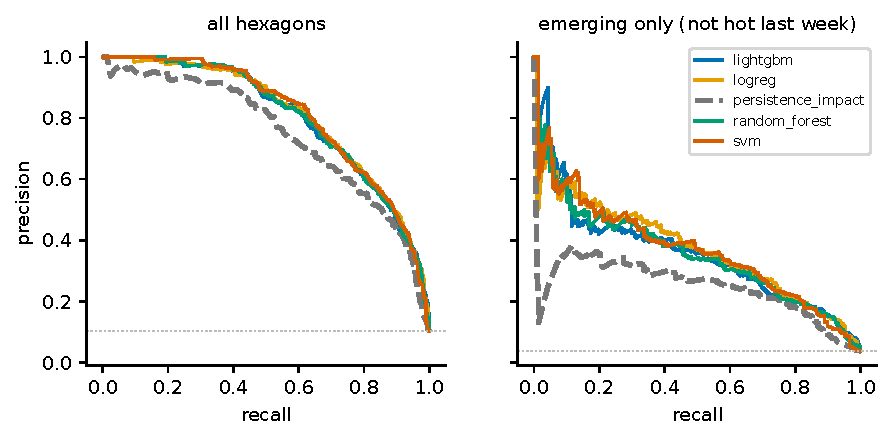
\includegraphics[width=\columnwidth]{E4_pr_curves}
\caption{Precision-recall curves pooled over four test blocks; the dashed line is persistence by impact.}
\label{fig:pr}
\end{figure}

\subsection{Training Loss Against Epochs}
Only the boosted model has an iterative training loop; the other models are fitted by closed-form or convex solvers with no epochs. Figure~\ref{fig:loss} therefore shows the training and validation loss of LightGBM against the boosting round, which plays the role of the epoch, on the last fold of each task (validation is the last 14 days or 2 weeks of the training window, the same split used for tuning). For counts the Poisson deviance of the training set keeps falling to 8.25 after 800 rounds, while the validation deviance bottoms out at 12.35 near round 223 and then rises to 12.98; for hotspots the log-loss minimum is 0.130 at round 104 against a training loss that keeps falling to 0.082. Both curves overfit slowly rather than sharply: by round 800 the validation deviance is only 5\% above its minimum. The tuned number of rounds (400 or 800 for counts, 50 for hotspots) is chosen on MAE and PR-AUC, not on this loss, so it can differ from the loss minimum.

\begin{figure*}[t]
\centering
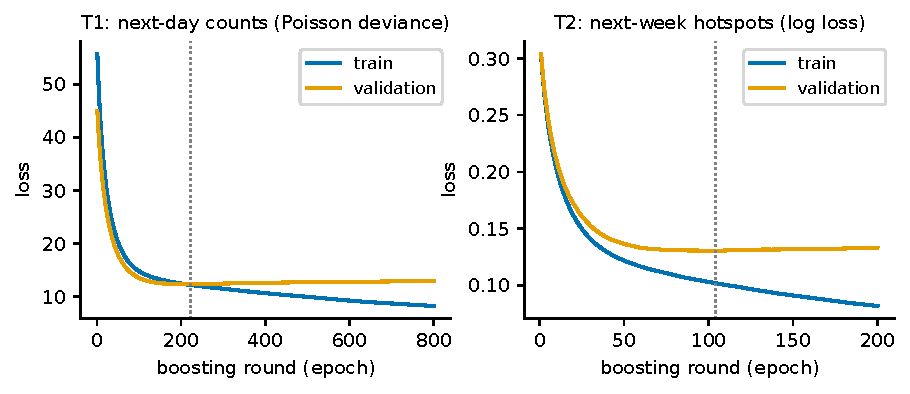
\includegraphics[width=0.8\textwidth]{F5_training_curve}
\caption{LightGBM training and validation loss against boosting round on the last fold. The dotted line marks the validation minimum.}
\label{fig:loss}
\end{figure*}

\subsection{Ablation Studies}
\textbf{Feature groups (T1, lasso).} Removing the history features (lags, rolling means, same-weekday mean) raises macro MASE from 0.697 to 0.746 (\(+0.048\)); removing the calendar flags (\(-0.003\)) or the station (\(+0.001\)) changes nothing outside the noise, so most of the signal is a station's recent level, which is why the moving average comes close. \textbf{Weight cap (E2).} The cap sweep of Table~\ref{tab:bench} and Figure~\ref{fig:bench} is the ablation of the benchmark: moving the cap from 2 to none trades bias\(^2\) from \(4.6\times10^{5}\) to 485 for variance from 122 to 17{,}817. \textbf{Volume term.} Against 12 expert-ranked junctions, the volume term of the impact score alone has Spearman \(\rho=0.93\) and the full score 0.92, so the extra terms add no agreement with the expert order.

\subsection{Uncertainty (E5)}
Table~\ref{tab:conf} reports 80\% split-conformal intervals around the lasso forecast. A single global interval is correct on average (80.3\%) but hides a large imbalance: 95\% coverage for low-volume stations and only 61\% for high-volume ones. Per-tier intervals give 79\%, 80\% and 82\%, at the cost of much wider bands where the counts are large (86 tickets instead of 44 for the busiest tier, 11 instead of 28 for the quietest). The mean absolute error is 5.8 tickets for the low tier and 30.0 for the high tier, which explains why one quantile cannot fit all.

\begin{table}[t]
\centering
\caption{80\% conformal intervals for next-day counts: coverage (\%) / mean width (tickets) by station-volume tier; target coverage 80\%.}
\label{tab:conf}
\footnotesize
\tab{conf}
\end{table}

\section{Conclusion}
Tickets record where officers were, and in Bengaluru officers almost disappear in the evening. A semi-synthetic benchmark shows how much that matters: naive counts miss 78\% of tickets, weighting needs the true exposure and a large cap, the cap that looks safe (12) leaves a \(-42\%\) bias, and an exposure curve estimated from the same thinned tickets does no better than the naive count. Forecasting is easier than recovery: a lasso on \(\log(1{+}y)\) forecasts next-day station counts at macro MASE 0.697 against 0.967 for the weekly baseline, and four classifiers rank next-week hotspots at PR-AUC about 0.80 against 0.743 for last week's impact, with linear models matching trees on both tasks. These models predict where tickets will be written, not where violations occur. Limitations: five months of one city and four folds; no congestion ground truth (the impact score is a proxy); a zero count can mean ``no violation'' or ``no officer''; the benchmark's truth window is itself slightly censored, so it measures recovery of a reference; timestamps may carry an offset; and our macro MASE is not comparable with the hackathon's pooled 0.73. Future work is exposure estimators that do not reuse the censored tickets, and applying the weighted target to real data.

\section*{Contributions}
Shaurya built the data layer, leak-free features, the evening-gap evidence and the unsupervised study. Afzal built the model comparison and reproducibility pipeline and the ParkSight hackathon baseline on which this work builds. Khushi designed and ran the censoring benchmark. Abdul built the metrics, conformal intervals, stratified error analysis, figure style and the report assembly.

\bibliographystyle{IEEEtran}
\bibliography{refs}

\end{document}
